%-------------------------
% Resume in Latex
% Author : Srinivas Rao Tammireddy
% LinkedIn: https://github.com/srinu2003/LaTex-Resume
% Based off of: https://www.overleaf.com/latex/templates/jakes-resume-anonymous/cstpnrbkhndn
% License : MIT
%------------------------

% \documentclass[letterpaper,11pt]{article}
\documentclass[a4paper,11pt]{article}

\usepackage{latexsym}
\usepackage[empty]{fullpage}
\usepackage{titlesec}
\usepackage{marvosym}
\usepackage[usenames,dvipsnames]{color}
\usepackage{verbatim}
\usepackage{enumitem}
\usepackage[hidelinks]{hyperref}
\usepackage{fancyhdr}
\usepackage[english]{babel}
\usepackage{tabularx}
\usepackage{fontawesome5}
\usepackage{multicol}
% \usepackage{fourier} % or \usepackage{newtxtext}
\usepackage{bold-extra}

\usepackage{graphicx}                       % For including graphics and images
\usepackage[export]{adjustbox}              % For positioning images 
\setlength{\multicolsep}{-3.0pt}
\setlength{\columnsep}{-1pt}
\input{glyphtounicode}

%----------FONT OPTIONS----------
% sans-serif
% \usepackage[sfdefault]{FiraSans}
% \usepackage[sfdefault]{roboto}
% \usepackage[sfdefault]{noto-sans}
% \usepackage[default]{sourcesanspro}

% serif
% \usepackage{CormorantGaramond}
% \usepackage{charter}

\pagestyle{fancy}
\fancyhf{} % clear all header and footer fields
\fancyfoot{}
\renewcommand{\headrulewidth}{0pt}
\renewcommand{\footrulewidth}{0pt}

% Adjust margins
% \addtolength{\oddsidemargin}{-0.5in}
% \addtolength{\evensidemargin}{-0.5in}
% \addtolength{\textwidth}{1in}
% \addtolength{\topmargin}{-.5in}
% \addtolength{\textheight}{1.0in}

\addtolength{\oddsidemargin}{-0.6in}
\addtolength{\evensidemargin}{-0.5in}
\addtolength{\textwidth}{1.19in}
\addtolength{\topmargin}{-.7in}
\addtolength{\textheight}{1.4in}

\urlstyle{same}

\raggedbottom
\raggedright
\setlength{\footskip}{4.08003pt}
\setlength{\tabcolsep}{0in}

% Sections formatting
\titleformat{\section}{
  %For bold small caps in Subheadings
  % \vspace{-4pt}\scshape\raggedright\large\bfseries 
  % For normal small caps in Subheadings
  \vspace{-6pt}\scshape\raggedright\large 
}{}{0em}{}[\color{black}\titlerule \vspace{-5pt}]

% Ensure that generate pdf is machine readable/ATS parsable
\pdfgentounicode=1

%-------------------------
% Custom commands
\newcommand{\resumeItem}[1]{\item\small{{#1 \vspace{-2pt}}}}
\newcommand{\classesList}[4]{\item\small{{#1 #2 #3 #4 \vspace{-2pt}}}}

\newcommand{\resumeSubheading}[4]{
  \vspace{-2pt}\item
    \begin{tabular*}{0.97\textwidth}[t]{l@{\extracolsep{\fill}}r}
      \textbf{#1} & \textbf{\small #2} \\
      \textit{\small#3} & \textit{\small #4} \\
    \end{tabular*}\vspace{-7pt}
}

\newcommand{\resumeSubSubheading}[2]{
  \item
    \begin{tabular*}{0.97\textwidth}{l@{\extracolsep{\fill}}r}
      \textit{\small#1} & \textit{\small #2} \\
    \end{tabular*}\vspace{-7pt}
}

\newcommand{\resumeProjectHeading}[2]{
  \item
    \begin{tabular*}{0.97\textwidth}{l@{\extracolsep{\fill}}r}
      \small#1 & \textbf{\small #2} \\
    \end{tabular*}\vspace{-7pt}
}

\newcommand{\resumeSubItem}[1]{\resumeItem{#1}\vspace{-4pt}}

\renewcommand\labelitemi{$\vcenter{\hbox{\tiny$\bullet$}}$}
\renewcommand\labelitemii{$\vcenter{\hbox{\tiny$\bullet$}}$}

\newcommand{\resumeSubHeadingListStart}{\begin{itemize}[leftmargin=0.15in, label={}]}
\newcommand{\resumeSubHeadingListEnd}{\end{itemize}}
\newcommand{\resumeItemListStart}{\begin{itemize}}
\newcommand{\resumeItemListEnd}{\end{itemize}\vspace{-5pt}}

% \usepackage{bold-extra} for bold small caps in section titles and subheadings. Instead of \normalshape, use \scshape in:
% \textbf{\Huge \normalshape Your Name} \\ \vspace{1pt}

%-------------------------------------------
%%%%%%  RESUME STARTS HERE  %%%%%%%%%%%%%%%%%%%%%%%%%%%%


\begin{document}

% %----------HEADING----------
% \begin{tabular*}{\textwidth}{l@{\extracolsep{\fill}}r}
%   \textbf{\href{http://srinu2003.me/}{\Large Srinivas Rao T}} & Email : \href{mailto:tsrin2003@gmail.com}{tsrin2003@gmail.com}\\
%   \href{http://srinu2003.me/}{http://www.srinu2003.me} & Mobile : +91 918-272-1417 \\
% \end{tabular*}

\begin{center}
    \begin{minipage}{0.7\textwidth}
        \raggedright
        {\Huge \scshape Srinivas Rao Tammireddy} \\ \vspace{6pt}
        Chintal, Hyderabad, Telangana 500054 \\ \vspace{1pt}
        \small
        \begin{itemize}[leftmargin=0.15in, label={}]
            \item \faPhone\ +91 918-272-1417
            \item \href{mailto:tsrin2003@gmail.com}{\faEnvelope\  {tsrin2003@gmail.com}}
            \item \href{https://linkedin.com/in/srinu2003/}{\faLinkedin\ {linkedin.com/in/srinu2003}}
            \item \href{https://github.com/srinu2003}{\faGithub\ {github.com/srinu2003}}
            % \item \href{https://www.youtube.com/@srinu.2003}{\faYoutube\ {youtube.com/@srinu.2003}}
        \end{itemize}
    \end{minipage}%
    \begin{minipage}{0.3\textwidth}
        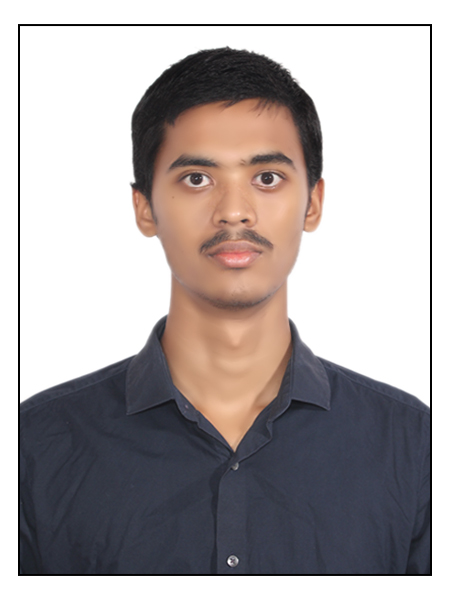
\includegraphics[width=3cm, center]{passport-size-photo.jpg}
    \end{minipage}
\end{center}


%-----------OBJECTIVE-----------
\section{Objective}
  \begin{itemize}[leftmargin=0.15in, label={}]
    \item \fontsize{10}{12} {\selectfont
    I am a \textbf{Computer Science Engineering} student at MLRITM, Hyderabad, passionate about \textbf{learning} new technologies and developing software applications. I strive to work on challenging assignments that offer job satisfaction and steady \textbf{professional growth}.}
  \end{itemize}

%-----------EDUCATION-----------
\vspace{-15pt}
\section{Education}
  \resumeSubHeadingListStart
    \resumeSubheading
      {\href{https://mlritm.ac.in}{Marri Laxman Reddy Institute of Technology and Management}}{Nov. 2021 -- Present}
      {B.Tech - Computer Science and Engineering, 8.94(Current)/10 CGPA}{Hyderabad, IND}
    \resumeSubheading
      {Sri Chaitanya Junior College}{June 2019 -- Apr. 2021}
      {Science with Maths, 94.8\% Higher Secondary, JEE (Main) 2021 - 81.70 percentile}{Hyderabad, IND}
    \resumeSubheading
      {Siddhartha High School}{Apr. 2019}
      {Secondary School, 9.7/10 CGPA}{Chintal, Hyderabad}
  \resumeSubHeadingListEnd

%------RELEVANT COURSEWORK-------
\section{Relevant Coursework}
        \begin{multicols}{4}
            \begin{itemize}[itemsep=-3pt, parsep=3pt]
              \small
                \item Data Structures
                \item Database Management
                \item Algorithms Analysis
                \item Applied Mathematics
                % \item Computer Architecture
                \item Operating Systems
                \item Software Engineering
                % \item Computer Networks
                % \item Blockchain
                \item Web Technologies
                \item Cryptography
              \end{itemize}
        \end{multicols}
        \vspace*{2.0\multicolsep}

% To be included in EXPERIENCE section if needed
% -----------Multiple Positions Heading-----------
%    \resumeSubSubheading
%     {Software Engineer I}{Oct 2014 - Sep 2016}
%     \resumeItemListStart
%        \resumeItem{Apache Beam}
%          {Apache Beam is a unified model for defining both batch and streaming data-parallel processing pipelines}
%     \resumeItemListEnd
%-------------------------------------------

%-----------EXPERIENCE-----------
\section{Experience}
    \resumeSubHeadingListStart
        \resumeSubheading
            {\href{https://g.dev/tsrinu2003}{Programming Lead}}{June 2023 -- June 2024}
            {Google Developers Students Club}{MLRITM, Dundigal}
            \resumeItemListStart
                \resumeItem{Mentored juniors, improving their technical skills with Google Developer Tools.}
                \resumeItem{Organized workshops and bootcamps, fostering a collaborative learning environment.}
        \resumeItemListEnd
        \resumeSubheading
            {\href{http://kitsltd.co.uk/index.html}{Software Engineer Assistant Intern}}{July 2024 -- June 2025}
            {Keertana Information Technology Solutions Limited}{KITS Ltd, UK}
            \resumeItemListStart
                \resumeItem{Developing and maintaining databases for company projects, ensuring optimal performance.}
                \resumeItem{Collaborating with the development team to implement new features and functionalities.}
                \resumeItem{Assisting in the development of web portals (Kits-HRMS, Kist-AP, Kits-IHP) with databasea and backend support.}
                \resumeItem{Developing an Analatics Portal (Kits-ADAT) as part of company's product development.}
        \resumeItemListEnd
    \resumeSubHeadingListEnd

%-----------COMPETITIONS & HACKATHONS-----------
\section{Competitions \& Hackathons}
    \resumeSubHeadingListStart
        \resumeSubheading
            {\href{https://drive.google.com/file/d/1M_5k71Pplh6leoRYhYY6SjMcuziMO_Cd/view?usp=sharing}{UI/UX Hackathon}}{Sep. 2021}
            {MLRITM Department of C.S.E}{MLRITM, Dundigal}
            \resumeItemListStart
                \resumeItem{Designed adaptive UI/UX for cross-platform applications based on Material Design principles.}
        \resumeItemListEnd

        \resumeSubheading
            {Kavach 2023}{Apr. 2023}
            {Innovation \& Incubation Center}{MLRITM, Dundigal}
            \resumeItemListStart
                \resumeItem{Participated in a 24-hour hackathon to develop a real-world problem-solving solution.}
        \resumeItemListEnd
    \resumeSubHeadingListEnd

%-----------PROJECTS-----------
\section{Projects}
    \resumeSubHeadingListStart
    \resumeProjectHeading
      {\href{https://github.com/srinu2003/ibcm}{{\textbf{IBCM: Image-Based Construction Monitoring}} $|$ \emph{Python, Flask, React}}}{Jan 19, 2025 -- Present}
      \resumeItemListStart \vspace{0pt}
      \resumeItem{Developed a web application for monitoring construction progress using images.}
      \resumeItem{Enabled users to upload construction site images, analyze them using image processing techniques, and generate insights on construction progress.}
      \resumeItem{Provided features to compare progress with schedules and view detailed progress reports.}
    \resumeItemListEnd
      \resumeProjectHeading
          {\href{https://github.com/srinu2003/Magpie}{{\textbf{Magpie}} $|$ \emph{Python, Tkinter}}}{Feb 12, 2024 -- May 15, 2024}
          \resumeItemListStart \vspace{0pt}
          \resumeItem{Developed a Python application using the Tkinter library for Encrypting \& Decrypting files.}
          \resumeItem{Implemented a command line interface (CLI) and implemented symmetric encryption (SHA-256) and hashing techniques using cryptography.fernet library.}
          \resumeItemListEnd
      \resumeProjectHeading
        {\href{https://github.com/srinu2003/quote_of_the_day}{{\textbf{Quote of the Day}} $|$ \emph{Flutter, Dart}}}{April 29, 2024 -- Present}
        \resumeItemListStart
          \resumeItem{Developing a mobile application that shows quotes of the day.(Pre release was done on 6th Aug 2024)}
          \resumeItem{Implementing share features and data storage and following Material-3 Design for UI/UX.}
        \resumeItemListEnd
    \resumeSubHeadingListEnd

% In next page
\newpage

%-----------TECHNICAL SKILLS-----------
\section{Technical Skills}
 \begin{itemize}[leftmargin=0.15in, label={}]
    \small{\item{
     \textbf{Technical Languages}{: Java(Core), Python, Dart, C Language, *C\#, *SQL, HTML \& *CSS} \\
     \textbf{Developer Tools}{: MySQL Workbench, Jira, Git, Github, Visual Studio Code, *Linux, JetBrains PyCharm, Star UML, Jupyter Notebook, *MS Excel, MS Word, MySQL.} \\
     \textbf{Technologies/Frameworks}{: Flutter, Material-3 Design, \LaTeX, Streamlit, *Flask, *Blockchain, *Machine Learning} \\
    }}
  \begin{tabular*}{0.97\textwidth}[t]{l@{\extracolsep{\fill}}r}
    \textit{} & \textit{\small *Elementary proficiency} \\
  \end{tabular*}
  \vspace{-7pt}
 \end{itemize}

%-----------CODING PROFILES-----------
\vspace{-12pt}
\section{Coding Profiles}
\begin{multicols}{2}
  \begin{itemize}[leftmargin=0.15in, label={}]
    \small{\item{
      \href{https://leetcode.com/tsrin2003/}{\underline{\textbf{Leetcode}}{:} @tsrin2003} 1,448 (Max Rating) \\
      \href{https://www.hackerrank.com/tsrin2003}{\underline{\textbf{HackerRank}}{:} @tsrin2003} C-Programming \\
      \href{https://www.interviewbit.com/profile/srinu2003/}{\underline{\textbf{InterviewBit}}{:} @srinu2003} 130638 (Global Rank) \\
      \href{https://www.codechef.com/users/srinu2003}{\underline{\textbf{CodeChef}}{:} @srinu2003} 1,641 (Max Rating) [3 Star] \\
      \href{https://codeforces.com/profile/srinu2003}{\underline{\textbf{Codeforces}}{:} @srinu2003} 858 (max. newbie, 858) \\
      }
    }
  \end{itemize}
\end{multicols}

%-----------CERTIFICATIONS/COURSES-----------
\vspace{-3pt}
  \section{Certifications/Courses}
    \resumeItemListStart[parsep = 0pt]
      \resumeItem{\href{https://drive.google.com/file/d/1ciuy0EC8fBujuxVOcZ--oUG9OZ8eHr5D/view?usp=drive_link}
                        {\textbf{PCAP: Programming Essentials in Python} by Cisco \faExternalLink*} (Jul. 2022)}
      \resumeItem{\href{https://drive.google.com/file/d/1w72XSRwblf5AqqEBGvnUbvUayJTcpWO-/view?usp=drive_link}
                        {\textbf{Cisco Network Academy certification} by Essential and Advanced C \faExternalLink*} (Aug. 2022)}
      \resumeItem{\href{https://www.udemy.com/certificate/UC-79138624-8361-423b-b131-42765a08db12/}
                        {\textbf{Python: The Professional Guide For Beginners (2024 Edition)} by \href{https://www.linkedin.com/in/federicoazzu/}{Federico Azzurro} \faExternalLink*} (May. 2024)}
      \resumeItem{\href{https://www.hackerrank.com/certificates/607a2d4d88f1}
                        {\textbf{Python (Basic) certification} by HackerRank \faExternalLink*} (May. 2024)}
    \resumeItemListEnd

%-----------CONTRIBUTIONS-----------
\section{Contributions}
  \resumeSubHeadingListStart
    \resumeSubheading
      {Lab Manual Preparation}{Jul 12, 2024, -- Present}
      {Skill Development Course (UI Design with Flutter)}{MLRITM, Dundigal}
      \resumeItemListStart
        \resumeItem{Authored and designed a comprehensive lab manual covering topics like Flutter and Dart SDK installation, widgets, responsive UIs, state management, animations, REST API integrations, and unit testing.}
        \resumeItem{Ensured alignment with academic outcomes and provided additional resources for self-paced learning.}
        \resumeItem{Integrated official references from \href{https://flutter.dev}{Flutter Documentation}, \href{https://material.io}{Material Design Guidelines}, and third-party tools.}
          \resumeItem{\href{https://github.com/srinu2003/Flutter-Lab}{GitHub Repository Link: Flutter-Lab}}
              \resumeItemListEnd
          \resumeSubHeadingListEnd

%-----------INVOLVEMENT---------------
\vspace{-11pt}
\section{Honors and Awards}
  \resumeItemListStart[parsep = -2pt]
    \resumeItem{\textbf{Top 1} in Internal Coding Contest(Data Structures and Algorithms) conducted by Smart-Interviews, MLRITM}
    \resumeItem{\textbf{Top 2} in Bugbounty Contest in Tech Fest conducted at MLRITM}
  \resumeItemListEnd

%-------------------------------------------
\end{document}